\documentclass{article}
%--PASTE INTO MAIN FILE--
% \documentclass{article}
% %--PASTE INTO MAIN FILE--
% \documentclass{article}
% %--PASTE INTO MAIN FILE--
% \documentclass{article}
% \input{TexBase/DocumentBase.tex}
% \end{document}

\usepackage[margin = 0.7in]{geometry}
\usepackage{graphicx}
\usepackage{graphics}
\usepackage[T1]{fontenc}
\usepackage[polish]{babel}
\usepackage{cmap}
\usepackage[utf8]{inputenc}
\usepackage{float}
\usepackage{tabularx}
\usepackage[table,xcdraw]{xcolor}
\usepackage{lipsum}
\usepackage{titlesec}
\usepackage{minted}
\usepackage{xcolor}
\usepackage{caption}
\usepackage{enumitem}
\usepackage{csvsimple}
\usepackage{natbib}
\usepackage{blindtext}

\usepackage{amsmath} %math

\usepackage{numprint} % rounding
\usepackage[round-precision=3,round-mode=figures, scientific-notation=true]{siunitx} %scientific notation

\usepackage[hidelinks]{hyperref}
\usepackage{url}

\usepackage{bm} %bold for math


%TABS
\usepackage[]{booktabs}
\usepackage{tabularray}
\usepackage{multirow}

%\title{}
\author{Michał Dziedziak}
\date{\today}


\titlespacing\section{0pt}{12pt plus 4pt minus 2pt}{0pt plus 2pt minus 2pt}
\titlespacing\subsection{0pt}{12pt plus 4pt minus 2pt}{0pt plus 2pt minus 2pt}
\titlespacing\subsubsection{0pt}{12pt plus 4pt minus 2pt}{0pt plus 2pt minus 2pt}
\setlength{\parskip}{\baselineskip}%
\setlength{\parindent}{0pt}%

\newcommand{\squeezeup}{\vspace{-5mm}}


\begin{document}

\begin{titlepage}
    \begin{center}
        \vspace*{5cm}
        \rule{500pt}{1pt}\\
        \vspace*{0.5cm}
        \LARGE
        \textbf{Inżyniera Obrazów}\\
        \Large
        Laboratorium numer 2
        \vspace*{0.5cm}
        \rule{500pt}{1pt}
    \end{center}

    \vspace*{10cm}

    {\raggedright
        \large
        \textbf{Autor sprawozdania:} Michał Dziedziak 263901\\
        \textbf{Imię i Nazwisko prowadzącego kurs:} dr inż. Jan Nikodem\\
        \textbf{Dzień i godzina zajęć:} czwartek, 11:15 - 14:15
    }
\end{titlepage}


\tableofcontents
% \listoftables

%\renewcommand\listoflistingscaption{List of source codes}
% \listoflistings

\listoffigures


\newpage


% \begin{table}[H]
%     \centering
%     \begin{tabular}{|c|c|c|c|}%
%         \hline
%         \bfseries Numer iteracji & \bfseries Czas zalezienia rozwiązania [ms] & Koszt ścieżki & Błąd względny% specify table head
%         \csvreader[head to column names]{Csv/BestPathTest_SimulatedAnnealing_LINEAR_ftv47.csv}{}% use head of csv as column names
%         {\\\hline\Iteration & \num{\TimeInMiliSeconds} & \Cost & \num[round-precision=2, round-mode=places, scientific-notation=false]{\Error}\%}% specify your columns here
%         \\\hline    
%     \end{tabular}
%     \caption{}
%     \label{tab:}
% \end{table}

% \begin{figure}[H]
%     \centering
%     \resizebox{\columnwidth}{!}{%
%     \includegraphics{}%
%     }
%     \caption{}
%     \label{fig:}
% \end{figure}

% \begin{listing}[H]
%     \begin{minted}[frame=single,framesep=2mm,linenos,fontsize=\footnotesize]{language}
%         some code
%     \end{minted}
%     \caption{}
%     \label{lst:}
% \end{listing}


% \bibliographystyle{plainnat}
% \bibliography{TexBase/Bibliography}

% \end{document}

\usepackage[margin = 0.7in]{geometry}
\usepackage{graphicx}
\usepackage{graphics}
\usepackage[T1]{fontenc}
\usepackage[polish]{babel}
\usepackage{cmap}
\usepackage[utf8]{inputenc}
\usepackage{float}
\usepackage{tabularx}
\usepackage[table,xcdraw]{xcolor}
\usepackage{lipsum}
\usepackage{titlesec}
\usepackage{minted}
\usepackage{xcolor}
\usepackage{caption}
\usepackage{enumitem}
\usepackage{csvsimple}
\usepackage{natbib}
\usepackage{blindtext}

\usepackage{amsmath} %math

\usepackage{numprint} % rounding
\usepackage[round-precision=3,round-mode=figures, scientific-notation=true]{siunitx} %scientific notation

\usepackage[hidelinks]{hyperref}
\usepackage{url}

\usepackage{bm} %bold for math


%TABS
\usepackage[]{booktabs}
\usepackage{tabularray}
\usepackage{multirow}

%\title{}
\author{Michał Dziedziak}
\date{\today}


\titlespacing\section{0pt}{12pt plus 4pt minus 2pt}{0pt plus 2pt minus 2pt}
\titlespacing\subsection{0pt}{12pt plus 4pt minus 2pt}{0pt plus 2pt minus 2pt}
\titlespacing\subsubsection{0pt}{12pt plus 4pt minus 2pt}{0pt plus 2pt minus 2pt}
\setlength{\parskip}{\baselineskip}%
\setlength{\parindent}{0pt}%

\newcommand{\squeezeup}{\vspace{-5mm}}


\begin{document}

\begin{titlepage}
    \begin{center}
        \vspace*{5cm}
        \rule{500pt}{1pt}\\
        \vspace*{0.5cm}
        \LARGE
        \textbf{Inżyniera Obrazów}\\
        \Large
        Laboratorium numer 2
        \vspace*{0.5cm}
        \rule{500pt}{1pt}
    \end{center}

    \vspace*{10cm}

    {\raggedright
        \large
        \textbf{Autor sprawozdania:} Michał Dziedziak 263901\\
        \textbf{Imię i Nazwisko prowadzącego kurs:} dr inż. Jan Nikodem\\
        \textbf{Dzień i godzina zajęć:} czwartek, 11:15 - 14:15
    }
\end{titlepage}


\tableofcontents
% \listoftables

%\renewcommand\listoflistingscaption{List of source codes}
% \listoflistings

\listoffigures


\newpage


% \begin{table}[H]
%     \centering
%     \begin{tabular}{|c|c|c|c|}%
%         \hline
%         \bfseries Numer iteracji & \bfseries Czas zalezienia rozwiązania [ms] & Koszt ścieżki & Błąd względny% specify table head
%         \csvreader[head to column names]{Csv/BestPathTest_SimulatedAnnealing_LINEAR_ftv47.csv}{}% use head of csv as column names
%         {\\\hline\Iteration & \num{\TimeInMiliSeconds} & \Cost & \num[round-precision=2, round-mode=places, scientific-notation=false]{\Error}\%}% specify your columns here
%         \\\hline    
%     \end{tabular}
%     \caption{}
%     \label{tab:}
% \end{table}

% \begin{figure}[H]
%     \centering
%     \resizebox{\columnwidth}{!}{%
%     \includegraphics{}%
%     }
%     \caption{}
%     \label{fig:}
% \end{figure}

% \begin{listing}[H]
%     \begin{minted}[frame=single,framesep=2mm,linenos,fontsize=\footnotesize]{language}
%         some code
%     \end{minted}
%     \caption{}
%     \label{lst:}
% \end{listing}


% \bibliographystyle{plainnat}
% \bibliography{TexBase/Bibliography}

% \end{document}

\usepackage[margin = 0.7in]{geometry}
\usepackage{graphicx}
\usepackage{graphics}
\usepackage[T1]{fontenc}
\usepackage[polish]{babel}
\usepackage{cmap}
\usepackage[utf8]{inputenc}
\usepackage{float}
\usepackage{tabularx}
\usepackage[table,xcdraw]{xcolor}
\usepackage{lipsum}
\usepackage{titlesec}
\usepackage{minted}
\usepackage{xcolor}
\usepackage{caption}
\usepackage{enumitem}
\usepackage{csvsimple}
\usepackage{natbib}
\usepackage{blindtext}

\usepackage{amsmath} %math

\usepackage{numprint} % rounding
\usepackage[round-precision=3,round-mode=figures, scientific-notation=true]{siunitx} %scientific notation

\usepackage[hidelinks]{hyperref}
\usepackage{url}

\usepackage{bm} %bold for math


%TABS
\usepackage[]{booktabs}
\usepackage{tabularray}
\usepackage{multirow}

%\title{}
\author{Michał Dziedziak}
\date{\today}


\titlespacing\section{0pt}{12pt plus 4pt minus 2pt}{0pt plus 2pt minus 2pt}
\titlespacing\subsection{0pt}{12pt plus 4pt minus 2pt}{0pt plus 2pt minus 2pt}
\titlespacing\subsubsection{0pt}{12pt plus 4pt minus 2pt}{0pt plus 2pt minus 2pt}
\setlength{\parskip}{\baselineskip}%
\setlength{\parindent}{0pt}%

\newcommand{\squeezeup}{\vspace{-5mm}}


\begin{document}

\begin{titlepage}
    \begin{center}
        \vspace*{5cm}
        \rule{500pt}{1pt}\\
        \vspace*{0.5cm}
        \LARGE
        \textbf{Inżyniera Obrazów}\\
        \Large
        Laboratorium numer 2
        \vspace*{0.5cm}
        \rule{500pt}{1pt}
    \end{center}

    \vspace*{10cm}

    {\raggedright
        \large
        \textbf{Autor sprawozdania:} Michał Dziedziak 263901\\
        \textbf{Imię i Nazwisko prowadzącego kurs:} dr inż. Jan Nikodem\\
        \textbf{Dzień i godzina zajęć:} czwartek, 11:15 - 14:15
    }
\end{titlepage}


\tableofcontents
% \listoftables

%\renewcommand\listoflistingscaption{List of source codes}
% \listoflistings

\listoffigures


\newpage


% \begin{table}[H]
%     \centering
%     \begin{tabular}{|c|c|c|c|}%
%         \hline
%         \bfseries Numer iteracji & \bfseries Czas zalezienia rozwiązania [ms] & Koszt ścieżki & Błąd względny% specify table head
%         \csvreader[head to column names]{Csv/BestPathTest_SimulatedAnnealing_LINEAR_ftv47.csv}{}% use head of csv as column names
%         {\\\hline\Iteration & \num{\TimeInMiliSeconds} & \Cost & \num[round-precision=2, round-mode=places, scientific-notation=false]{\Error}\%}% specify your columns here
%         \\\hline    
%     \end{tabular}
%     \caption{}
%     \label{tab:}
% \end{table}

% \begin{figure}[H]
%     \centering
%     \resizebox{\columnwidth}{!}{%
%     \includegraphics{}%
%     }
%     \caption{}
%     \label{fig:}
% \end{figure}

% \begin{listing}[H]
%     \begin{minted}[frame=single,framesep=2mm,linenos,fontsize=\footnotesize]{language}
%         some code
%     \end{minted}
%     \caption{}
%     \label{lst:}
% \end{listing}


% \bibliographystyle{plainnat}
% \bibliography{TexBase/Bibliography}


\section{Zadanie 1 (zaległe 4)}
    \subsection{Cel zadania}
    Zadanie pierwsze (zaległe 4 z poprzedniej listy) polegało na przeprowadzeniu symulacji transmisji obrazu w 
    systemie DVB.

    W ramach tego zadania należało wykonać nasypujące kroki:
    \begin{enumerate}
        \item Przeprowadzić konwersję wybranego obrazy z modelu RGB do YCbCr
        \item Wykonac operacje \textit{downsamplingu} na kanałach Cb i Cr
        \item Wykonac operacje \textit{upsamplingu} na kanałach Cb i Cr
        \item Przeprowadzić konwersję odwrotną, z YCbCr do RGB
        \item Wyświetlić obraz przed i po wysłaniu, wraz ze składowymi Y, Cb i Cr
    \end{enumerate}

    \subsection{Teoria}
    \textbf{Model YCbCr} - Model ten jest modelem przestrzeni barw, który składa się z trzech składowych: Y,
    Cb i Cr. Składowa Y odpowiada za jasność, a składowe Cb i Cr za kolor. Dokładne omówienie modelu
    miało miejsce w poprzednim sprawozdaniu.

    \textbf{Downsampling} jest procesem zmniejszania częstotliwości próbkowania sygnału, co prowadzi 
    do redukcji ilości danych. W ramach tego procesu, próbki sygnału są usuwane lub pomijane, aby 
    zmniejszyć liczbę próbek w sygnale. Operacja downsamplingu jest często stosowana w celu zmniejszenia 
    rozmiaru danych lub zmniejszenia wymagań przepustowości, co może być korzystne w przypadku 
    transmisji danych przez ograniczone kanały komunikacyjne lub w celu redukcji mocy obliczeniowej 
    wymaganej do przetwarzania sygnału.

    \textbf{Upsampling}, również znany jako interpolacja, jest procesem zwiększania częstotliwości 
    próbkowania sygnału poprzez dodanie nowych próbek między istniejącymi. Głównym celem upsamplingu 
    jest przywrócenie oryginalnej rozdzielczości sygnału po jego zmniejszeniu w procesie downsamplingu 
    lub poprawa jakości sygnału poprzez dodanie informacji.
    W procesie upsamplingu, nowe próbki są wprowadzane między istniejące próbki sygnału, zwykle poprzez 
    interpolację wartości pomiędzy nimi. Istnieją różne techniki interpolacji stosowanych w upsamplingu, 
    np. interpolacja liniowa i interpolacja dwusześcienna.

    Źródła: \cite{Downsampling}, \cite{Upsampling}

    \subsection{Prezentacja wykonanego zadania}
    Operacja downsamplingu została wykonana poprzez pominięcie co drugiego piksela w kanałach Cb i Cr.
    Upsampling został wykonany poprzez powielenie każdego piksela wzdłuż obu osi w kanałach Cb i Cr.  
    
    \begin{figure}[H]
        \centering
        \resizebox{\columnwidth}{!}{%
        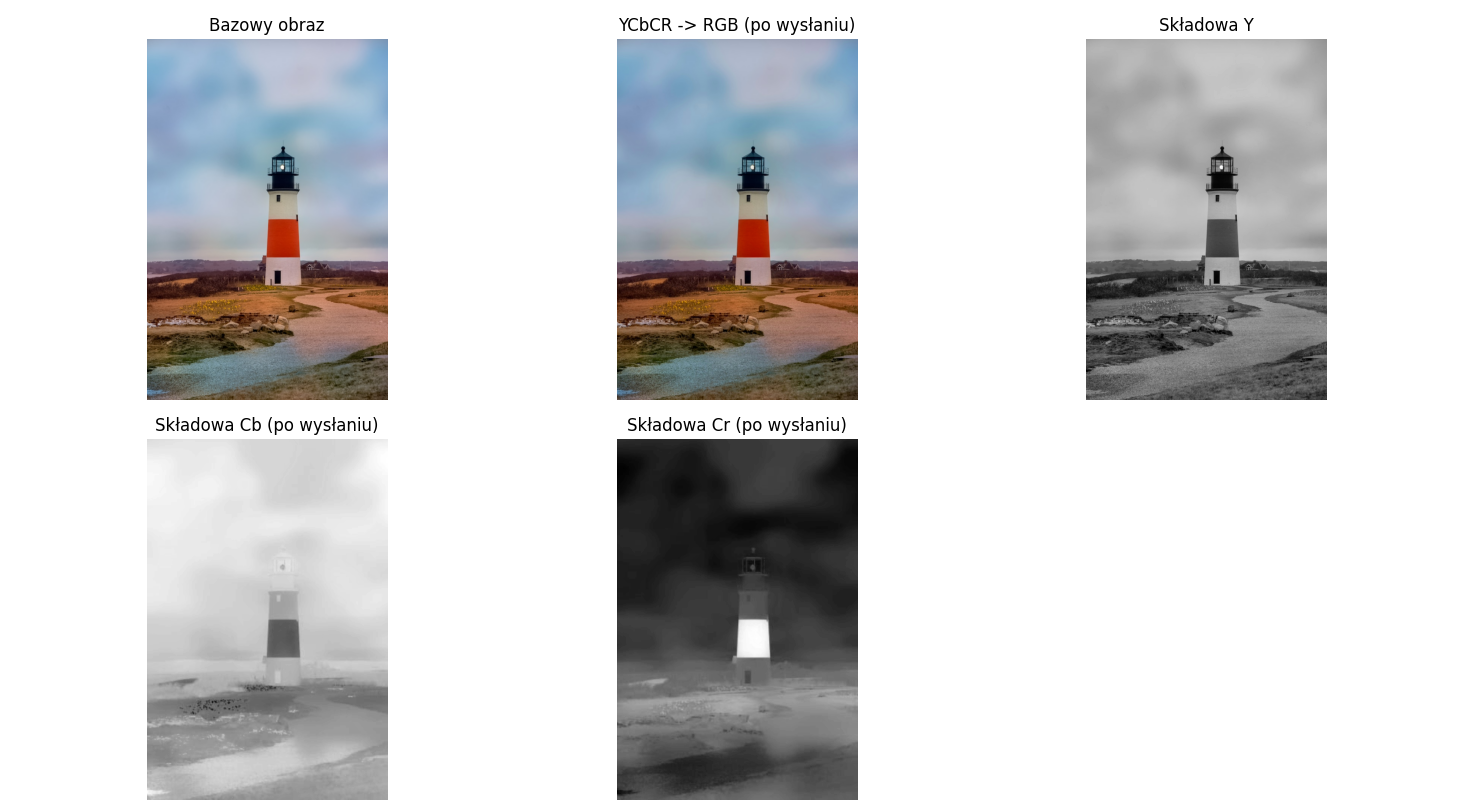
\includegraphics{Img/zad1z.png}%
        }
        \caption{Zdjęcie przedstawiające obraz przed i po przeprowadzeniu symulacji transmisji DVB}
        \label{fig:zad1z}
    \end{figure}


\section{Zadanie 2 (zaległe 5)}
    \subsection{Cel zadania}
    W ramach zaległego zadania piątego mieliśmy policzyć błąd średniokwadratowy
    pomiędzy: 
    \begin{itemize}
        \item obrazem oryginalnym (RGB), a obrazem po konwersji YCbCr
        \item obrazem oryginalnym (RGB), a obrazem po transmisji DVB
    \end{itemize}

    \subsection{Teoria}
    Błąd średniokwadratowy (MSE) jest miarą różnicy pomiędzy dwoma obrazami. Jest to
    jedna z najczęściej stosowanych miar jakości obrazu, która oblicza średnią kwadratów
    różnic pomiędzy pikselami dwóch obrazów. MSE jest obliczane zgodnie ze wzorem:
    \begin{equation}
        MSE = \frac{1}{n \cdot m} \sum_{i=0}^{n} \sum_{j=0}^{m} (X_{ij} - \hat{X}_{ij})^2
    \end{equation}
    gdzie:
    \begin{itemize}
        \item $X_{ij}$ - wartość piksela obrazu oryginalnego
        \item $\hat{X}_{ij}$ - wartość piksela obrazu wynikowego
        \item $n$ - liczba pikseli obrazu
        \item $m$ - liczba kanałów obrazu
    \end{itemize}

    \subsection{Prezentacja wykonanego zadania}
    Obrazy dla których liczony był błąd średniokwadratowy posiadały wartości pikseli z zakresu 0 - 255.

    \begin{figure}[H]
        \centering
        \resizebox{\columnwidth}{!}{%
        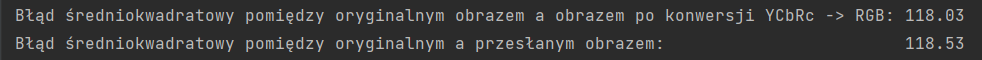
\includegraphics{Img/zad2z.png}%
        }
        \caption{Zdjęcie konsoli z obliczonymi wartościami MSE}
        \label{fig:zad2z}
    \end{figure}


\section{Zadanie 1}
    \subsection{Cel zadania}
    W ramach tego zadania mieliśmy zaimplementować obsługę plików ppm (format P3 i P6).
    
    Kolejne kroki:
    \begin{enumerate}
        \item Zapisać i odczytać szkic (mały, prosty obraz) w formacie P3 i P6
        \item Zapisać i odczytać obraz w formacie P3 i P6
        \item Porównać rozmiary plików
    \end{enumerate}

    \subsection{Teoria}
    \textbf{Pliki PPM} (Portable Pixmap Format) to format plików graficznych używany do przechowywania 
    obrazów w postaci mapy pikseli. Jest to format bezstratnej kompresji obrazu, 
    co oznacza, że nie powoduje utraty danych podczas zapisu i odczytu. 

    \textbf{PPM w formacie P3} jest zapisywany jako plik tekstowy, w którym wartości pikseli są 
    zapisane jako ciągi znaków ASCII. Każdy piksel jest opisany przez trzy liczby, reprezentujące 
    składowe koloru.  Pliki w formacie P3 są czytelne dla ludzi, ale zajmują więcej miejsca na 
    dysku w porównaniu do formatu binarnego. 

    \textbf{PPM w formacie P6} jest zapisywany jako plik binarny, w którym wartości pikseli są 
    zapisane w formie surowych bajtów. Podobnie jak w formacie P3, każdy piksel jest opisany 
    przez trzy bajty, reprezentujące składowe koloru. Pliki w formacie P6 zajmują mniej 
    miejsca na dysku niż format tekstowy P3.

    Źródła \cite{P3}, \cite{PPM}, \cite{PPM2}

    \subsection{Prezentacja wykonanego zadania}
    \begin{figure}[H]
        \centering
        \resizebox{\columnwidth}{!}{%
        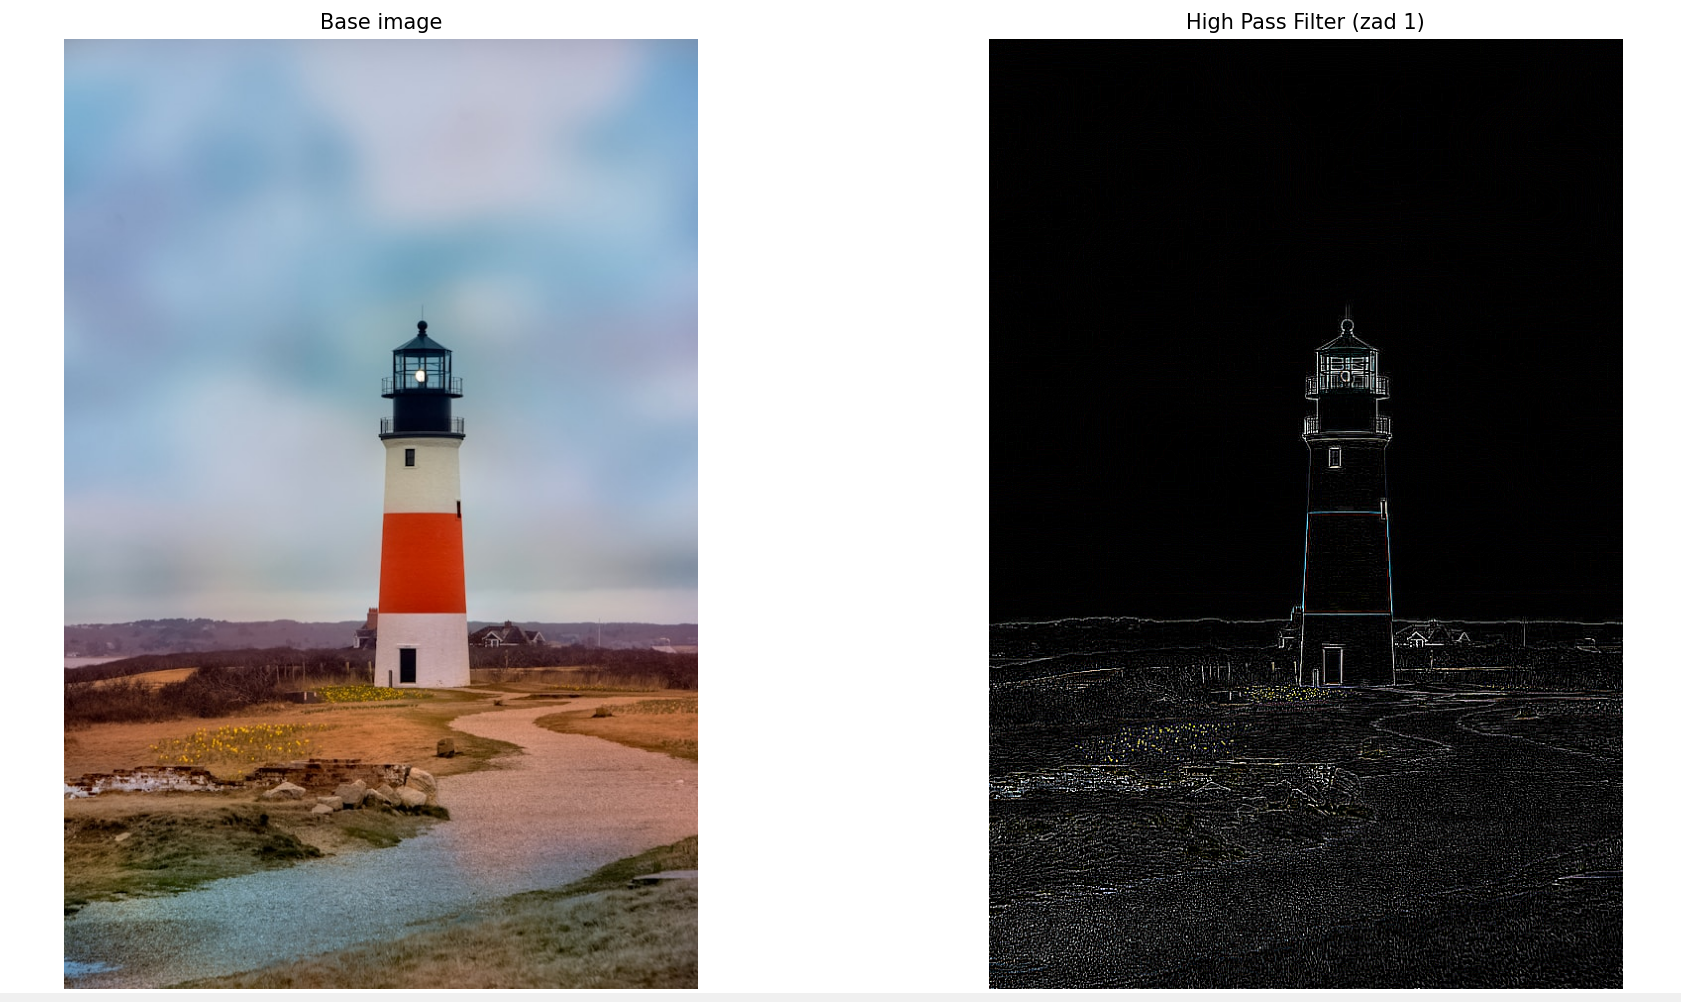
\includegraphics{Img/zad1.png}%
        }
        \caption{Prezentacja obrazów odczytanych z plików P3 i P6}
        \label{fig:zad1}
    \end{figure}

    \begin{figure}[H]
        \centering
        \resizebox{\columnwidth / 2}{!}{%
        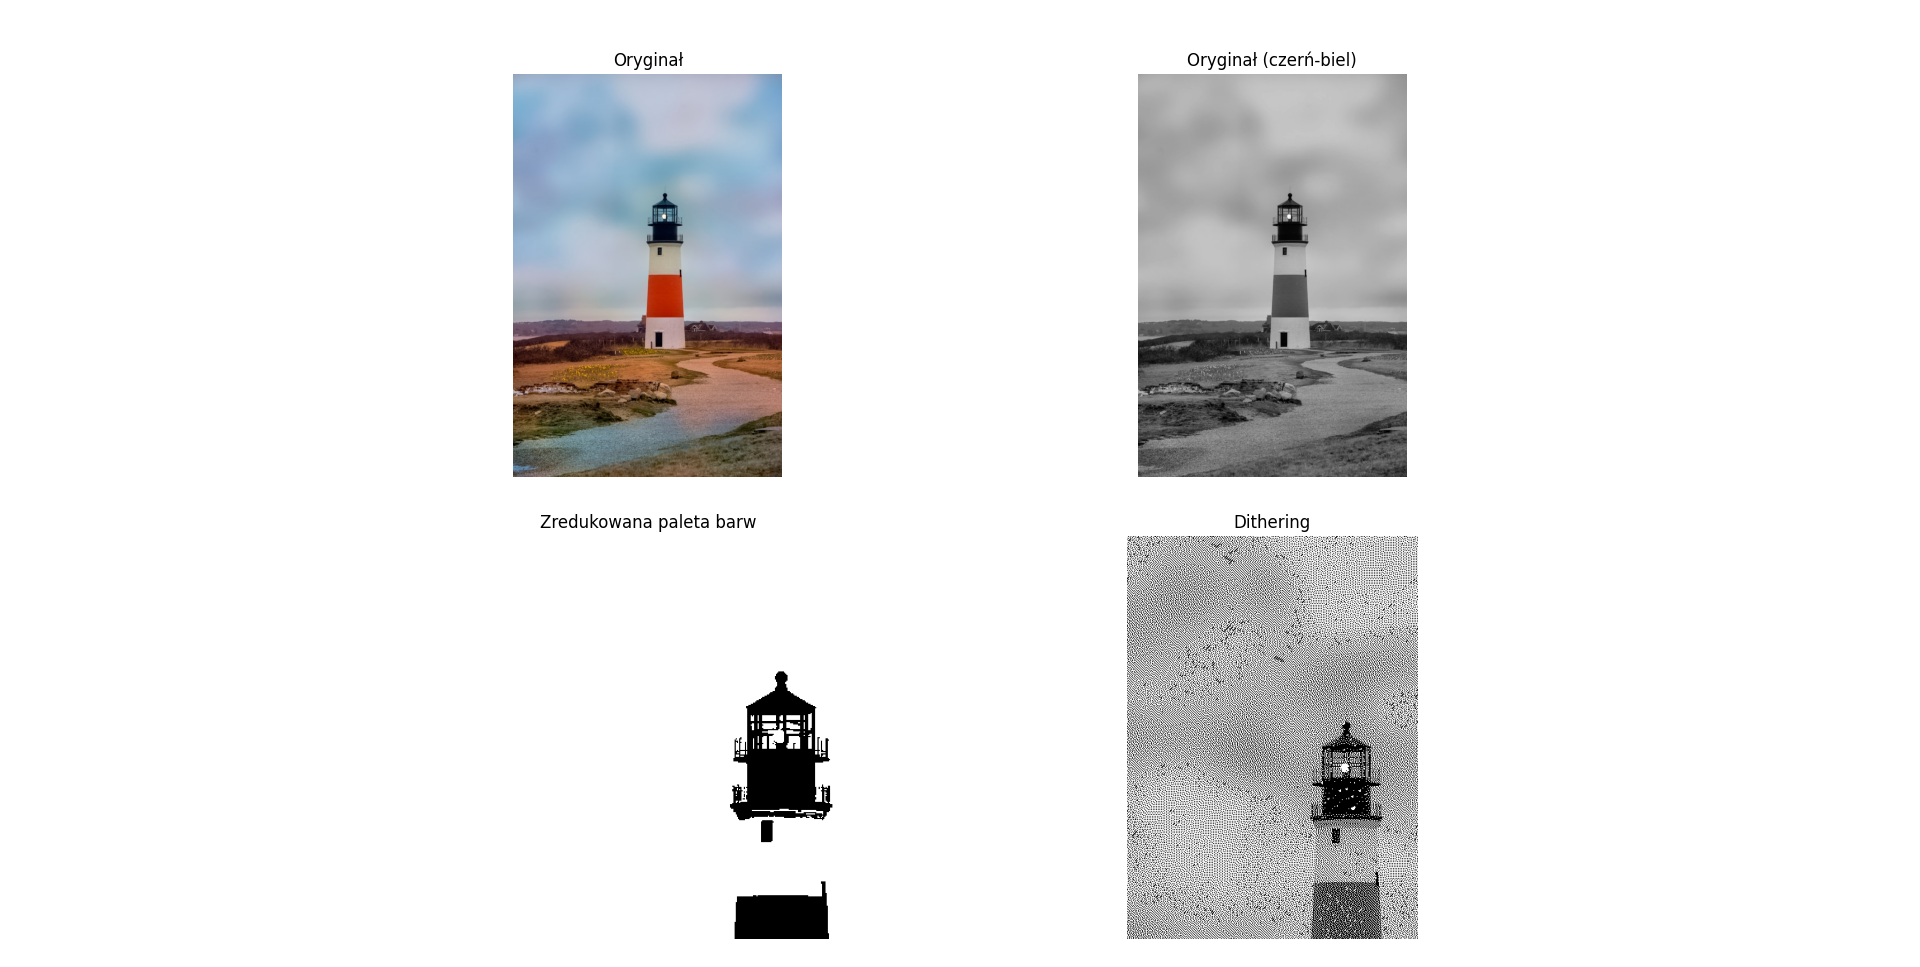
\includegraphics{Img/zad1_2.png}%
        }
        \caption{Zdjęcie konsoli z wypisanymi rozmiarami plików}
        \label{fig:zad1_2}
    \end{figure}

    \begin{figure}[H]
        \centering
        \resizebox{\columnwidth/2}{!}{%
        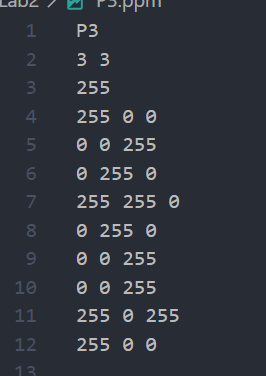
\includegraphics{Img/zad1_3.png}%
        }
        \caption{Zawartość pliku P3\_szkic}
        \label{fig:zad1_3}
    \end{figure}

    \begin{figure}[H]
        \centering
        \resizebox{\columnwidth/2}{!}{%
        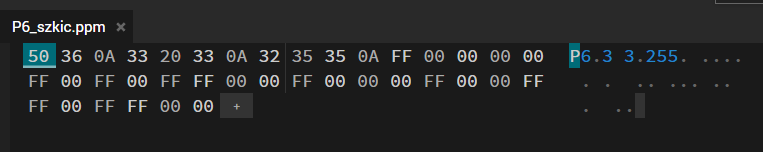
\includegraphics{Img/zad1_4.png}%
        }
        \caption{Zawartość pliku P6\_szkic}
        \label{fig:zad1_4}
    \end{figure}

    
\section{Zadanie 2}
    \subsection{Cel zadania}
    Celem zadania drugiego było umieszczenie schematu przestrzeni barw RGB w wybranym formacie pliku ppm. 
    W rezultacie mieliśmy otrzymać dwa spektra.
    Jedno czarno-białe i drugie wielokolorowe, wyglądające następująco:
    \begin{figure}[H]
        \centering
        \resizebox{\columnwidth}{!}{%
        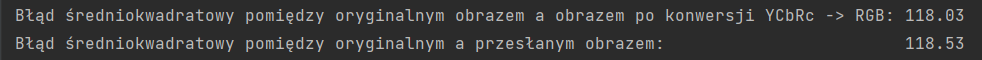
\includegraphics{Img/zad2z.png}%
        }
        \caption{Spektrum do uzyskania w zadaniu}
    \end{figure}

    \subsection{Prezentacja wykonanego zadania}
    Do zapisu plików ppm wykorzystano format P3.

    \begin{figure}[H]
        \centering
        \resizebox{\columnwidth}{!}{%
        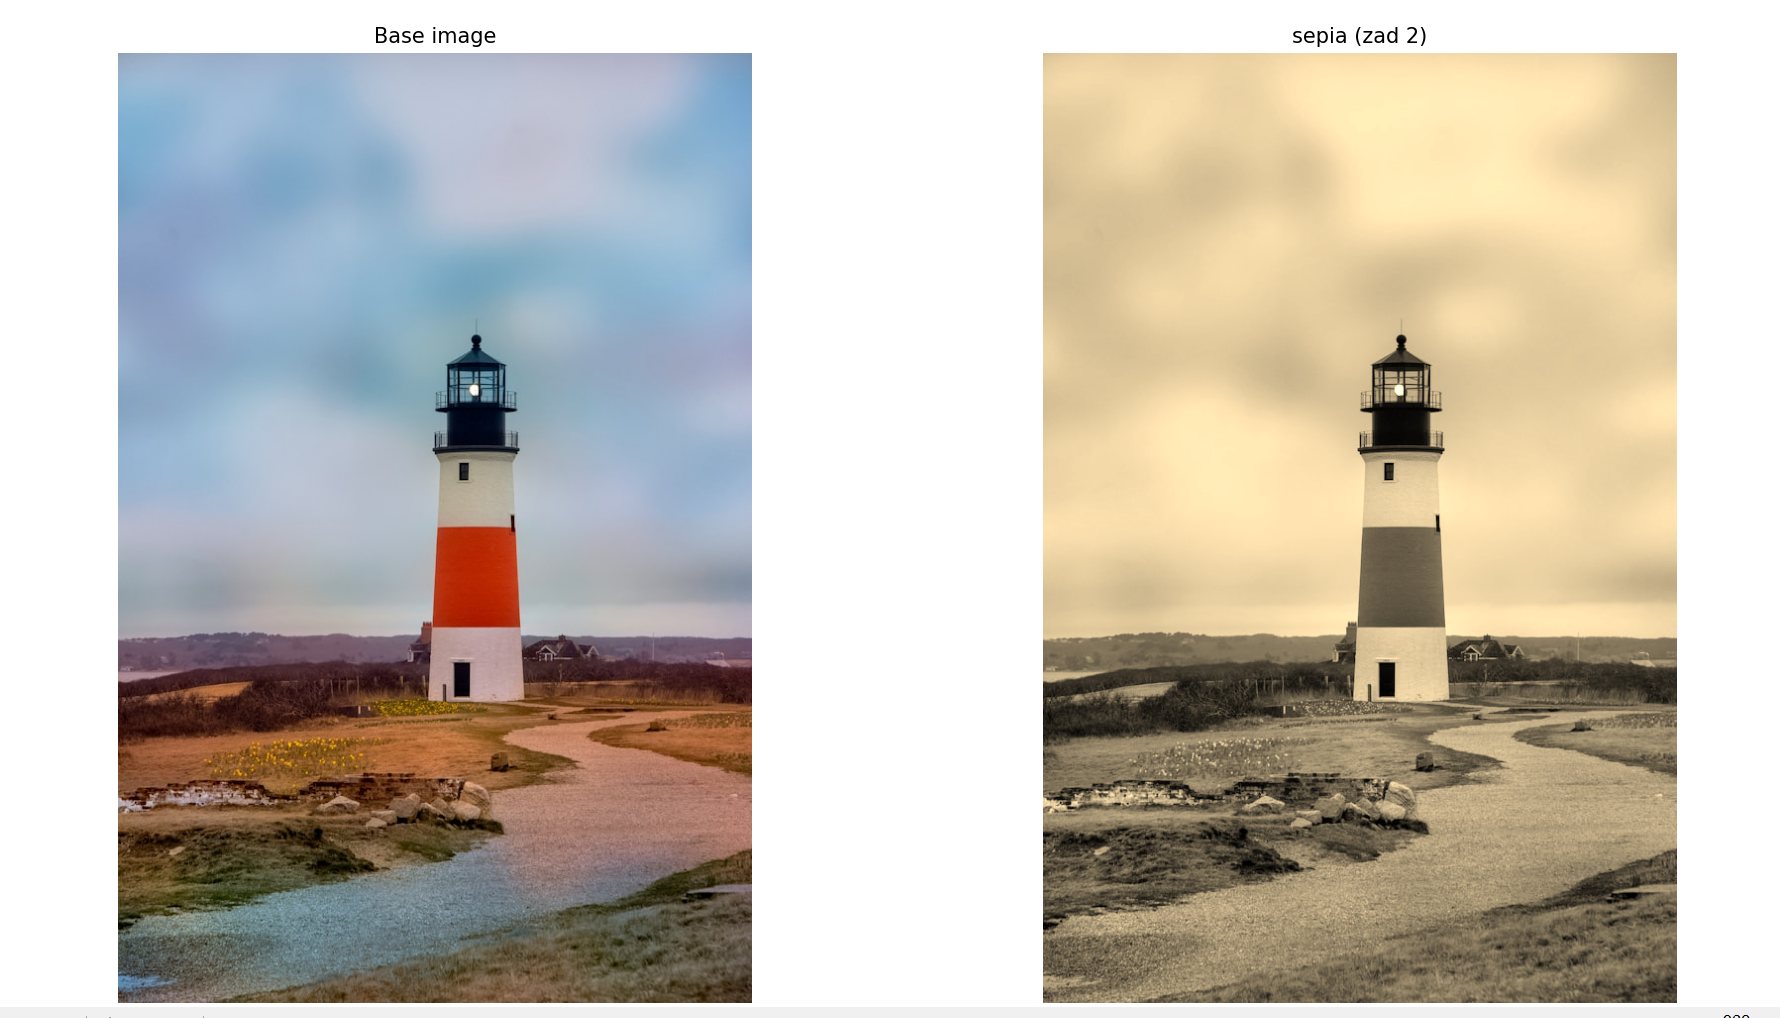
\includegraphics{Img/zad2.png}%
        }
        \caption{Zdjęcie przedstawiające oba spektra uzyskane w wyniku wykonania zadania}
    \end{figure}


\section{Zadanie 3}
    \subsection{Cel zadania}
    Celem zadania trzeciego było stworzenie zbioru graficznego w formacie PNG. 
    Wykorzystano obraz tęczy z poprzedniego ćwiczenia, tworząc wariant bez przezroczystości. 
    Utworzony obraz ma być możliwy do odczytania i wyświetlania w programie graficznym obsługującym PNG.

    \subsection{Teoria}
    Format plików PNG (Portable Network Graphics) jest formatem obrazów rastrowych. 
    Charakteryzuje się on zachowaniem przezroczystości oraz kompresją bezstratną.

        \subsubsection*{Nagłówek PNG}

        Początek każdego pliku PNG jest określony przez 8-bajtowy nagłówek. Specyficzna 
        sekwencja znaków, znana jako sygnatura: 137 80 78 71 13 10 26 10 (dziesiętne), identyfikuje plik jako format PNG.

        \subsubsection*{Chunki}

        Struktura plików PNG opiera się na "chunkach", które są to strukturami danych zdefiniowanymi przez specyfikację PNG. Każdy chunk składa się z czterech głównych części: długość danych, typ chunka, rzeczywiste dane oraz wartość CRC (Cyclic Redundancy Check) służąca do weryfikacji integralności danych. Chunki mogą reprezentować różne aspekty obrazu, takie jak informacje o nagłówku (IHDR), paleta kolorów (PLTE), rzeczywiste dane obrazu (IDAT) oraz końcowy znacznik (IEND).

        \subsubsection*{Strumień zlib}

        Wewnątrz chunka IDAT, dane obrazu są kompresowane za pomocą algorytmu DEFLATE, który jest częścią biblioteki zlib.

        \subsubsection*{Filtracja i tryby kompresji}

        W procesie kompresji wewnątrz chunka IDAT, każdy wiersz obrazu jest poddawany filtracji. Istnieje pięć dostępnych filtrów, które są stosowane w celu optymalizacji procesu kompresji i poprawy efektywności przechowywania danych obrazu.

    Źródła: \cite{PNG}

    \subsection{Prezentacja wykonanego zadania}
    \begin{figure}[H]
        \centering
        \resizebox{\columnwidth}{!}{%
        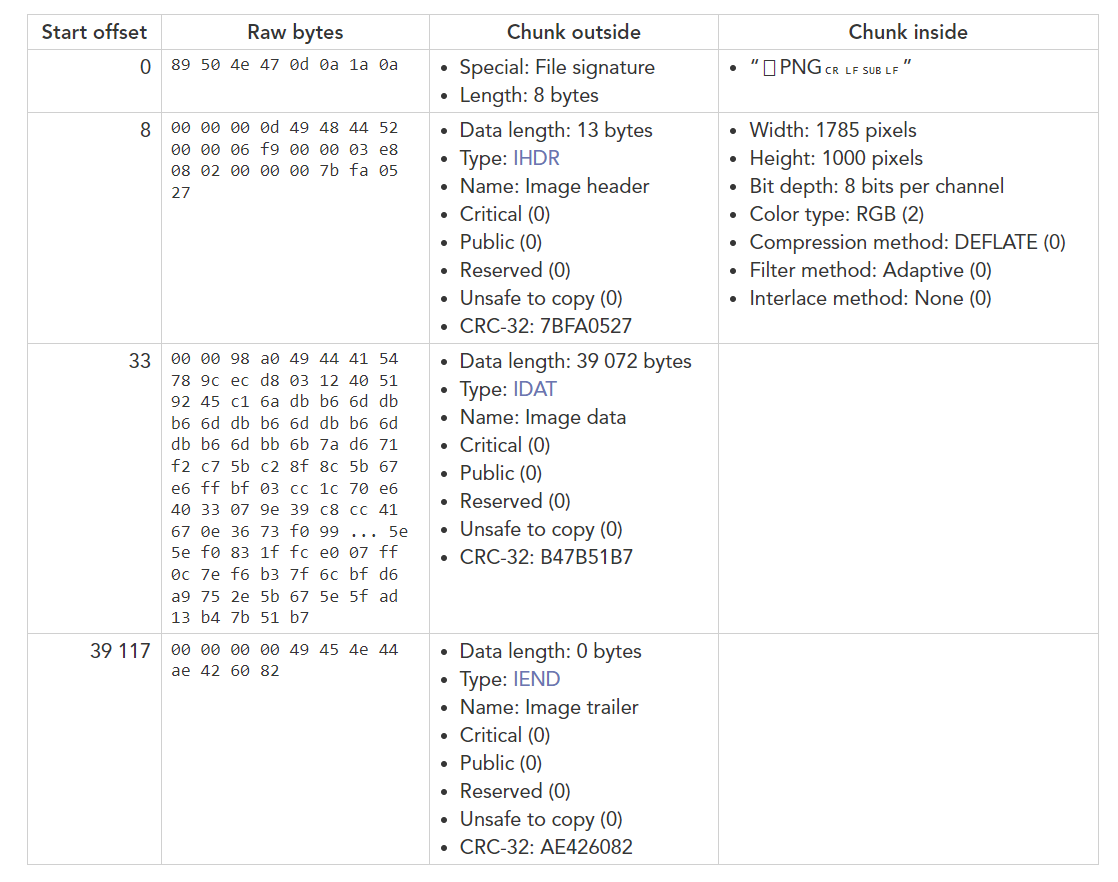
\includegraphics{Img/zad3_0.png}%
        }
        \caption{Zdjęcie przedstawiające strukturę stworzonego pliku PNG}
    \end{figure}

    \begin{figure}[H]
        \centering
        \resizebox{\columnwidth}{!}{%
        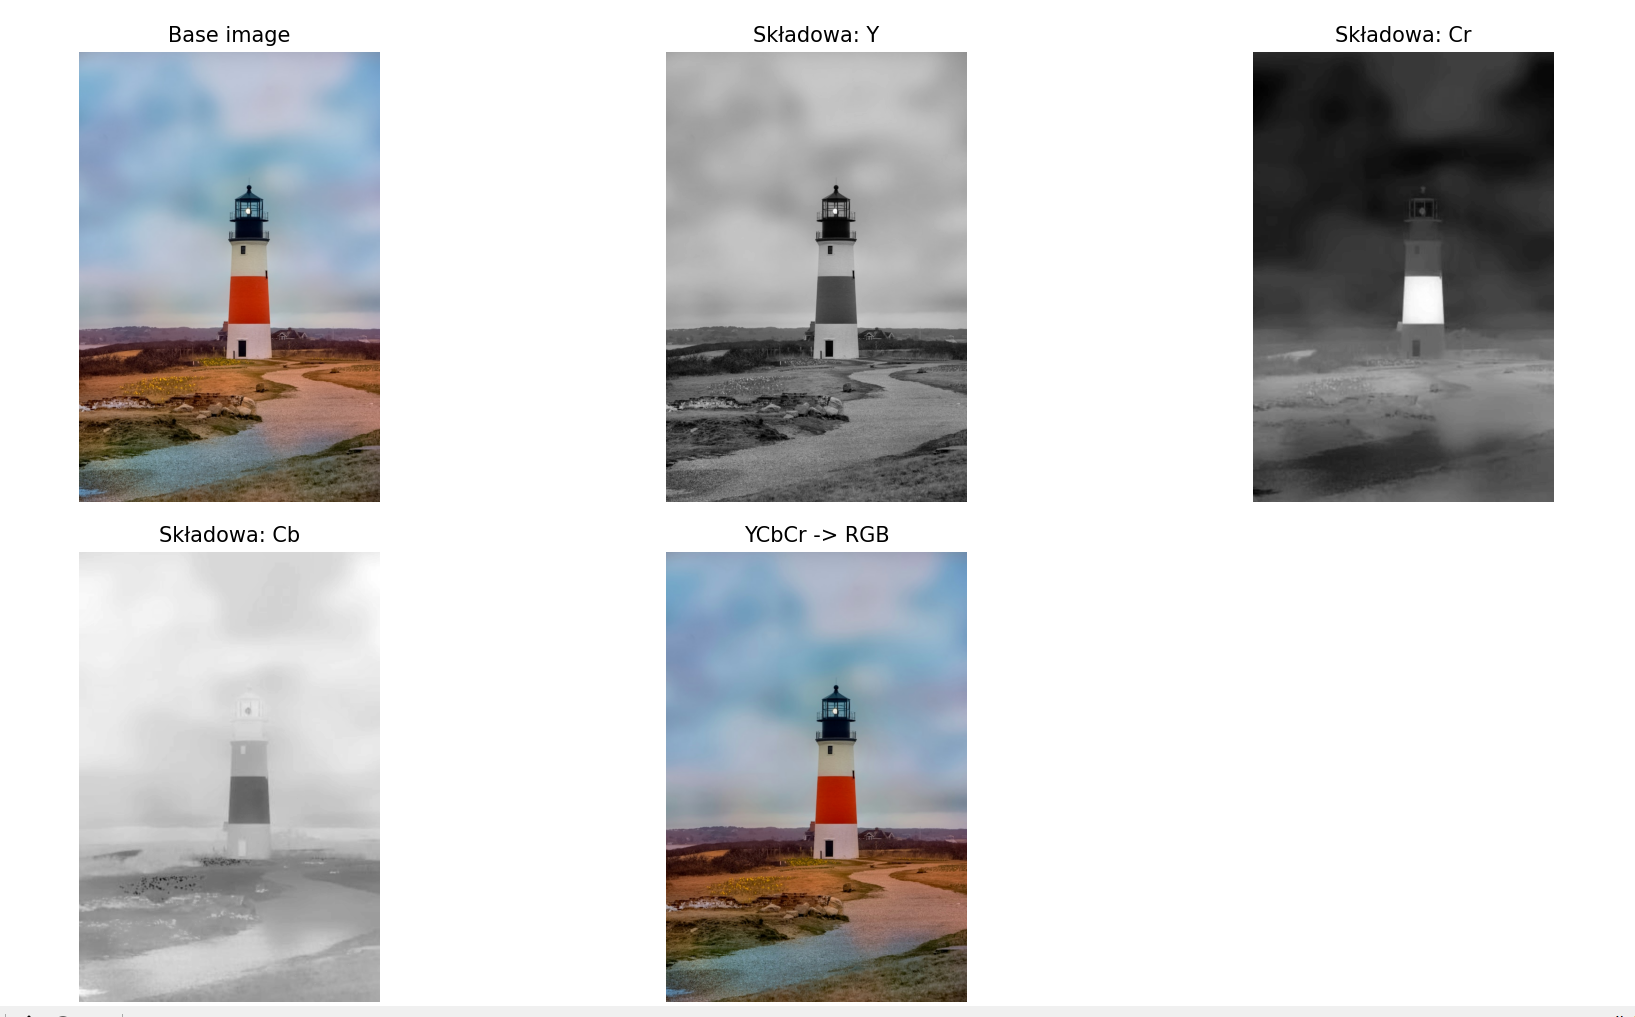
\includegraphics{Img/zad3.png}%
        }
        \caption{Zdjęcie przedstawiające odczytany plik PNG}
    \end{figure}
    


\bibliographystyle{plainnat}
\bibliography{TexBase/Bibliography}

\end{document}